\documentclass[xcolor=dvipsnames,table]{beamer}

\usepackage{latexsym}
\usepackage[utf8]{inputenc}
\usepackage[brazil]{babel}
\usepackage{amssymb}
\usepackage{amsmath}
\usepackage{stmaryrd}
\usepackage{fancybox}
\usepackage{datetime}
\usepackage[T1]{fontenc}
\usepackage{graphicx}
\usepackage{graphics}
\usepackage{url}
\usepackage{algorithmic}
\usepackage{algorithm}
\usepackage{acronym}
\usepackage{array}

\newtheorem{definicao}{Definio}
\newcommand{\tab}{\hspace*{2em}}

\mode<presentation>
{
  \definecolor{colortexto}{RGB}{0,0,0}
 
  \setbeamertemplate{background canvas}[vertical shading][ bottom=white!10,top=white!10]
  \setbeamercolor{normal text}{fg=colortexto} 

  \usetheme{Warsaw}
}

\title{Matrizes de Incidência e Adjacências} 

\author{
  Esdras Lins Bispo Jr. \\ \url{bispojr@ufg.br}
  } 
 \institute{
  Teoria de Grafos \\Bacharelado em Ciência da Computação}
\date{\textbf{10 de maio de 2017} }

\logo{
\includegraphics[width=1cm]{images/ufgJataiLogo.png}}

\begin{document}

	\begin{frame}
		\titlepage
	\end{frame}

	\AtBeginSection{
		\begin{frame}{Sumário}%[allowframebreaks]{Sumário}
    		\tableofcontents[currentsection]
    		%\tableofcontents[currentsection, hideothersubsections]
		\end{frame}
	}

	\begin{frame}{Plano de Aula}
		\tableofcontents
		%\tableofcontents[hideallsubsections]
	\end{frame}
    
    \begin{frame}{Pensamento}
		\begin{columns}
			\column{.4\textwidth}  		
		  		\begin{center}
		    		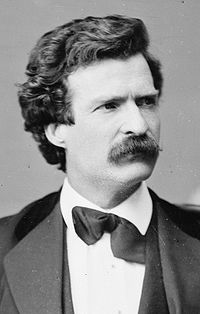
\includegraphics[height=.8\textheight]{images/mark.jpg}
		  		\end{center}
			\column{.6\textwidth}  		
				\begin{block}{Frase}
					\begin{center}
						{\large A gente não se liberta de um hábito atirando-o pela janela: é preciso fazê-lo descer a escada, degrau por degrau.}
					\end{center}
				\end{block}		  		
		  		\begin{block}{Quem?}
		  			\begin{center}
						{\bf Mark Twain (1835 - 1910)} \\Escritor e humorista estadunidense
					\end{center}
				\end{block}
		\end{columns}
	\end{frame}
    
    \section{Revisão}
	\subsection{Outras terminologias}
	\begin{frame}{Outras terminologias}
		\begin{block}{$V(G)$ e $A(G)$}
			Se o nome de um grafo for $G$, então o conjunto de seus vértices será denotado por $V(G)$ e o conjunto de suas arestas por $A(G)$.
		\end{block}
		\begin{block}{$n(G)$ e $m(G)$}
			O número de vértices de $G$ é denotado por $n(G)$ e o número de arestas por $m(G)$. 
		\end{block}
		\begin{block}{Corolário}
			$n(G) = |V(G)|$ e $m(G) = |A(G)|$.
		\end{block}
	\end{frame}
	
	\begin{frame}{Outras terminologias}
		\begin{block}{$\overline{G}$}
			O complemento de um grafo $(V, A)$ é o grafo $(V, V^{(2)} \setminus A)$.
		\end{block}
		\begin{block}{$K_n$} 
			O grafo $G$ é {\bf completo} se $A(G) = V(G)^{(2)}$. A expressão ``$G$ é um $K_n$'' é uma abreviatura de ``$G$ é um grafo completo com $n$ vértices''.
		\end{block}
		\begin{block}{$\overline{K_n}$} 
			O grafo $G$ é {\bf vazio} se $A(G) =\emptyset$. A expressão ``$G$ é um $\overline{K_n}$'' é uma abreviatura de ``$G$ é um grafo vazio com $n$ vértices''.
		\end{block}
	\end{frame}
    
    \subsection{Vizinhança}
	\begin{frame}{Vizinhança}
		\begin{block}{Vizinhança}
			\begin{itemize}
				\item A {\bf vizinhança} de um vértice $v$ em um grafo $G$ é o conjunto de todos os vizinhos de $v$;
				\item Este conjunto será denotado por $N_G(v)$ \\(ou simplesmente $N(v$)).
			\end{itemize}
		\end{block}
		\begin{exampleblock}{Lembrando...}
			Seja $G$ um grafo e $v, u \in V(G)$. \\Dizemos que $v$ é vizinho de $u$ se existe uma aresta que os liga.
		\end{exampleblock}
	\end{frame}
	
	\begin{frame}{Grau}
		\begin{block}{Grau}
			\begin{itemize}
				\item O {\bf grau} de um vértice $v$ em um grafo $G$ é o número de arestas que incidem em $v$; 
				\item Este valor será denotado por $d_G(v)$ (ou simplesmente $d(v$);
				\item Um vértice $v$ é {\bf isolado} se $d(v) = 0$.
			\end{itemize}
		\end{block}
		\begin{block}{Corolário}
			\begin{itemize}
				\item $d_G(v) = |N(v)|$.
			\end{itemize}
		\end{block}		
	\end{frame}
	
	\begin{frame}[shrink]{Grau mínimo e Grau máximo}
		\begin{block}{Grau mínimo}
			$\delta(G) :=  \underset{v \in V(G)}{min} d_G(v)$
		\end{block} 
		\begin{block}{Grau máximo}
			$\Delta(G) :=  \underset{v \in V(G)}{max} d_G(v)$
		\end{block}
		\begin{block}{Média dos graus}
			$\mu(G) =  \dfrac{1}{|V(G)|} \underset{v \in V(G)}{\sum} d_G(v)$
		\end{block} 
		\begin{block}{Corolário}
			$\mu(G) = \dfrac{2m(G)}{n(G)}$
		\end{block}
	\end{frame}
	
	\begin{frame}{Grafo regular}
		\begin{block}{Grafo regular}
			Um grafo é {\bf regular} se todos os seus vértices têm o mesmo grau, ou seja, se $\delta = \Delta$.
		\end{block} 
		\begin{block}{$r$-regular}
			Um grafo é $r$-regular se $d(v) = r$ para todo vértice $v$.
		\end{block} 
		\begin{block}{Grafo cúbico}
			Um {\bf grafo cúbico} é o mesmo que um grafo 3-regular.
		\end{block}
	\end{frame}

	\section{Matriz de adjacências e incidências}
	\begin{frame}{Matriz de adjacências e incidências}
		\begin{block}{Definição}
			Uma {\bf matriz de adjacências} de um grafo $G$ é a matriz $A$ definida da seguinte maneira: para todo vértice $u$ e $v$
			\begin{center}
				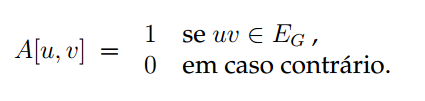
\includegraphics[width=.5\textwidth]{images/adjacencia.png}
			\end{center}
		\end{block} \pause
		\begin{block}{Definição}
			Uma {\bf matriz de incidências} de um grafo $G$ é a matriz $M$ definida da seguinte maneira: para todo vértice $u$ e uma aresta $e$
			\begin{center}
				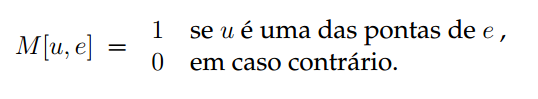
\includegraphics[width=.6\textwidth]{images/incidencia.png}
			\end{center}
		\end{block}
	\end{frame}
	
	\begin{frame}
		\titlepage
	\end{frame}
	
\end{document}